\begin{figure}[htb]
       \begin{center}
               \scalebox{0.9}{
                        \nonstopmode
                        % GNUPLOT: LaTeX picture with Postscript
\begingroup
  \makeatletter
  \providecommand\color[2][]{%
    \GenericError{(gnuplot) \space\space\space\@spaces}{%
      Package color not loaded in conjunction with
      terminal option `colourtext'%
    }{See the gnuplot documentation for explanation.%
    }{Either use 'blacktext' in gnuplot or load the package
      color.sty in LaTeX.}%
    \renewcommand\color[2][]{}%
  }%
  \providecommand\includegraphics[2][]{%
    \GenericError{(gnuplot) \space\space\space\@spaces}{%
      Package graphicx or graphics not loaded%
    }{See the gnuplot documentation for explanation.%
    }{The gnuplot epslatex terminal needs graphicx.sty or graphics.sty.}%
    \renewcommand\includegraphics[2][]{}%
  }%
  \providecommand\rotatebox[2]{#2}%
  \@ifundefined{ifGPcolor}{%
    \newif\ifGPcolor
    \GPcolortrue
  }{}%
  \@ifundefined{ifGPblacktext}{%
    \newif\ifGPblacktext
    \GPblacktexttrue
  }{}%
  % define a \g@addto@macro without @ in the name:
  \let\gplgaddtomacro\g@addto@macro
  % define empty templates for all commands taking text:
  \gdef\gplbacktext{}%
  \gdef\gplfronttext{}%
  \makeatother
  \ifGPblacktext
    % no textcolor at all
    \def\colorrgb#1{}%
    \def\colorgray#1{}%
  \else
    % gray or color?
    \ifGPcolor
      \def\colorrgb#1{\color[rgb]{#1}}%
      \def\colorgray#1{\color[gray]{#1}}%
      \expandafter\def\csname LTw\endcsname{\color{white}}%
      \expandafter\def\csname LTb\endcsname{\color{black}}%
      \expandafter\def\csname LTa\endcsname{\color{black}}%
      \expandafter\def\csname LT0\endcsname{\color[rgb]{1,0,0}}%
      \expandafter\def\csname LT1\endcsname{\color[rgb]{0,1,0}}%
      \expandafter\def\csname LT2\endcsname{\color[rgb]{0,0,1}}%
      \expandafter\def\csname LT3\endcsname{\color[rgb]{1,0,1}}%
      \expandafter\def\csname LT4\endcsname{\color[rgb]{0,1,1}}%
      \expandafter\def\csname LT5\endcsname{\color[rgb]{1,1,0}}%
      \expandafter\def\csname LT6\endcsname{\color[rgb]{0,0,0}}%
      \expandafter\def\csname LT7\endcsname{\color[rgb]{1,0.3,0}}%
      \expandafter\def\csname LT8\endcsname{\color[rgb]{0.5,0.5,0.5}}%
    \else
      % gray
      \def\colorrgb#1{\color{black}}%
      \def\colorgray#1{\color[gray]{#1}}%
      \expandafter\def\csname LTw\endcsname{\color{white}}%
      \expandafter\def\csname LTb\endcsname{\color{black}}%
      \expandafter\def\csname LTa\endcsname{\color{black}}%
      \expandafter\def\csname LT0\endcsname{\color{black}}%
      \expandafter\def\csname LT1\endcsname{\color{black}}%
      \expandafter\def\csname LT2\endcsname{\color{black}}%
      \expandafter\def\csname LT3\endcsname{\color{black}}%
      \expandafter\def\csname LT4\endcsname{\color{black}}%
      \expandafter\def\csname LT5\endcsname{\color{black}}%
      \expandafter\def\csname LT6\endcsname{\color{black}}%
      \expandafter\def\csname LT7\endcsname{\color{black}}%
      \expandafter\def\csname LT8\endcsname{\color{black}}%
    \fi
  \fi
  \setlength{\unitlength}{0.0500bp}%
  \begin{picture}(7680.00,7680.00)%
    \gplgaddtomacro\gplbacktext{%
      \colorrgb{0.00,0.00,0.00}%
      \put(866,845){\makebox(0,0)[r]{\strut{}0}}%
      \colorrgb{0.00,0.00,0.00}%
      \put(866,1627){\makebox(0,0)[r]{\strut{}500}}%
      \colorrgb{0.00,0.00,0.00}%
      \put(866,2410){\makebox(0,0)[r]{\strut{}1000}}%
      \colorrgb{0.00,0.00,0.00}%
      \put(866,3192){\makebox(0,0)[r]{\strut{}1500}}%
      \colorrgb{0.00,0.00,0.00}%
      \put(866,3974){\makebox(0,0)[r]{\strut{}2000}}%
      \colorrgb{0.00,0.00,0.00}%
      \put(866,4756){\makebox(0,0)[r]{\strut{}2500}}%
      \colorrgb{0.00,0.00,0.00}%
      \put(866,5539){\makebox(0,0)[r]{\strut{}3000}}%
      \colorrgb{0.00,0.00,0.00}%
      \put(866,6321){\makebox(0,0)[r]{\strut{}3500}}%
      \colorrgb{0.00,0.00,0.00}%
      \put(866,7103){\makebox(0,0)[r]{\strut{}4000}}%
      \colorrgb{0.00,0.00,0.00}%
      \put(998,625){\makebox(0,0){\strut{}0}}%
      \colorrgb{0.00,0.00,0.00}%
      \put(2486,625){\makebox(0,0){\strut{}50}}%
      \colorrgb{0.00,0.00,0.00}%
      \put(3974,625){\makebox(0,0){\strut{}100}}%
      \colorrgb{0.00,0.00,0.00}%
      \put(5462,625){\makebox(0,0){\strut{}150}}%
      \colorrgb{0.00,0.00,0.00}%
      \put(6950,625){\makebox(0,0){\strut{}200}}%
      \colorrgb{0.00,0.00,0.00}%
      \put(96,3974){\rotatebox{90}{\makebox(0,0){\strut{}\rule{0pt}{-1.5cm}CPU time in seconds to simulate one nanosecond.}}}%
      \colorrgb{0.00,0.00,0.00}%
      \put(3974,295){\makebox(0,0){\strut{}Number of boxes per dimension}}%
    }%
    \gplgaddtomacro\gplfronttext{%
    }%
    \gplbacktext
    \put(0,0){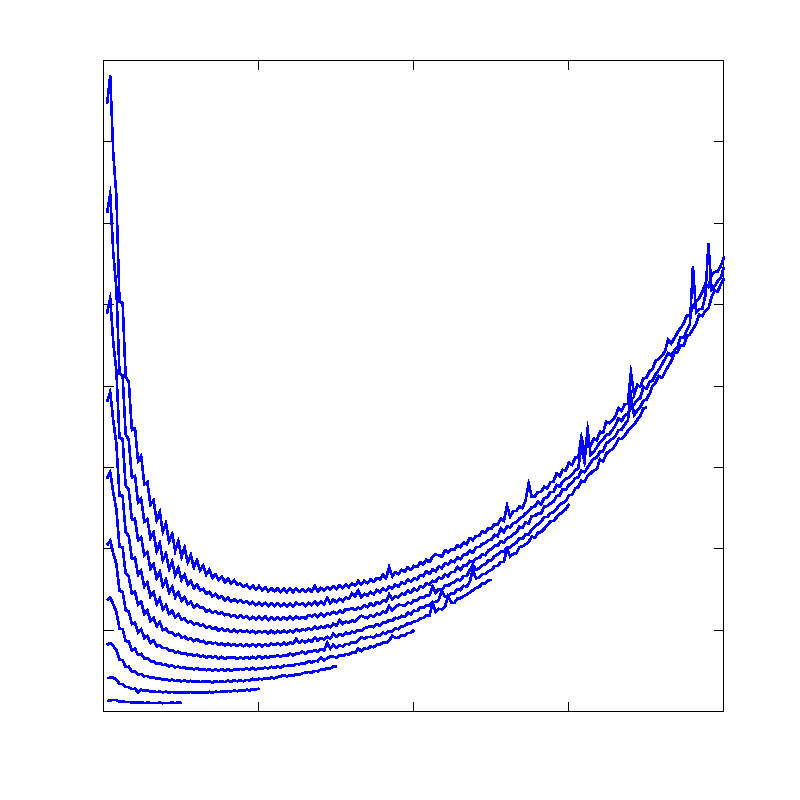
\includegraphics{images/performancePerNumBox}}%
    \gplfronttext
  \end{picture}%
\endgroup

                        \errorstopmode
                        \rule[-0.5cm]{0cm}{0cm}}
                \caption{Performance in function of the number of boxes for various strand lengths $N$ of ssDNA. The bottom curve corresponds to $N = 100$, each successively higher curve represents an additional 100 monomers, up to the top curve, where $N = 1000$.}
                \label{performancePerNumBox}
        \end{center}
\end{figure}

